\documentclass[12pt]{../oss-classkick-exam}
\usepackage{enumitem}
\usepackage{bm}

\begin{document}
\begin{center}
  \textbf{PHYSICS C: ELECTRICITY AND MAGNETISM\\
    Section I\\
    Time--45 minutes\\
    30 Questions
  }
\end{center}

\textbf{Directions:} Each of the questions or incomplete statements below is
followed by five suggested answers or completions. Select the one that is best
in each case and place the letter of your choice in the corresponding box on
the student answer sheet.

\begin{questions}
%  \question Two negative point charges are a distance $x$ apart and have
%  potential energy $U$. If the distance between the point charges increases to
%  $3x$, what is their new potential energy?
%  \begin{choices}
%    \choice $9U$
%    \choice $3U$
%    \choice $U$
%    \choice $U/3$
%    \choice $U/9$
%  \end{choices}
%
%  \uplevel{\rule{\linewidth}{.5pt}}
  
  \question An electric field is produced by the very long, uniformly charged
  rod drawn below. If the strength of the electric field is $E_1$ at a distance
  $r_1$ from the axis of the rod, at what distance from the axis is
  the field strength $E_1/4$?

  \vspace{.1in}
  \begin{minipage}{.35\linewidth}
    \pic{.85}{rod1}
  \end{minipage}
  \begin{minipage}{.4\linewidth}
    \begin{choices}
      \choice $r_1/4$
      \choice $r_1/2$
      \choice $2r_1$
      \choice $4r_1$
      \choice $16r_1$
    \end{choices}
  \end{minipage}
  
  \uplevel{
    \rule{\linewidth}{.5pt}
    
    \textbf{Question \ref{sphere1}--\ref{sphere2}}
    \begin{center}
      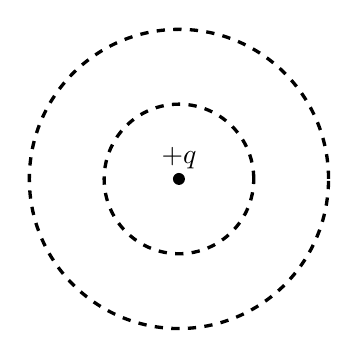
\begin{tikzpicture}[scale=.95]
        \fill circle(.08) node[above]{$+q$}; 
        \draw[very thick,dashed] circle(1);
        \draw[very thick,dashed] circle(2);
      \end{tikzpicture}
    \end{center}
    Two concentric spherical surfaces are drawn around an isolated positive
    charge $+q$ located at their center, as shown above. The inner surface has
    a radius that is $1/2$ that of the outer surface.
  }

  \question If the total electric flux passing through the inner surface is
  $\phi$, what is the total electric flux passing through the outer surface?
  \begin{choices}
    \choice $\phi/4$
    \choice $\phi/2$
    \choice $\phi$
    \choice $2\phi$
    \choice $4\phi$
  \end{choices}
  \label{sphere1}
  
  \question If the electric field strength at the inner surface is $E$, what is
  the electric field strength at the outer surface?
  \begin{choices}
    \choice $E/4$
    \choice $E/2$
    \choice $E$
    \choice $2E$
    \choice $4E$
  \end{choices}
  \label{sphere2}
  
  \uplevel{\rule{\linewidth}{.5pt}}
  
  \question Sphere $X$ of mass $M$ and charge $+q$ hangs from a string as shown
  below. Sphere $Y$ has an equal charge $+q$ and is fixed in place a distance
  $d$ directly below sphere $X$. If sphere $X$ is in equilibrium, the tension
  in the string is most nearly

  \begin{minipage}{.35\linewidth}
    \pic{.8}{2spheres}
  \end{minipage}
  \begin{minipage}{.5\linewidth}
    \begin{choices}
      \choice$Mg$
      \choice$Mg+\dfrac{kq}d$
      \choice$Mg-\dfrac{kq}d$
      \choice$Mg+\dfrac{kq^2}{d^2}$
      \choice$Mg-\dfrac{kq^2}{d^2}$
    \end{choices}
  \end{minipage}

  \uplevel{\rule{\linewidth}{.5pt}}
  
  \question A charge $+q$ is placed at the center of a tetrahedron whose faces
  are all equilateral triangles, as shown below. What is the flux of the
  electric field through one face of the tetrahedron?

  \begin{minipage}{.3\linewidth}
    \cpic{.67}{tetrahedral}
  \end{minipage}
  \begin{minipage}{.69\linewidth}
    \begin{choices}
      \choice 0
      \choice$q/\epsilon_0$
      \choice$q/4\epsilon_0$
      \choice$4\epsilon_0q$
      \choice The flux through one face cannot be determined from the
      information given.
    \end{choices}
  \end{minipage}
  \newpage
  
%  \question Two concentric metal spheres $X$ and $Y$ are shown above. $X$
%  carries a positive charge, and $Y$ is connected to ground. True statements
%  include which of the following?
%
%  \begin{minipage}{.3\linewidth}
%    \begin{tikzpicture}[scale=.95]
%      \begin{scope}[thick]
%        \draw circle(1.3);
%        \draw circle(2);
%        \draw(2,0)--(2.5,0)--(2.5,-1.5) node[ground]{};
%      \end{scope}
%      \node at (.8,.5) {$X$};
%      \node at (1.7,1.5) {$Y$};
%    \end{tikzpicture}
%  \end{minipage}
%  \begin{minipage}{.5\linewidth}
%    \vspace{.1in}
%    \begin{enumerate}[nosep,label=\Roman*.]
%    \item The electric field inside $X$ is zero.
%    \item The electric field outside $Y$ is zero.
%    \item The charge density on both spheres is the same.
%    \end{enumerate}
%
%    \vspace{.2in}\begin{choices}
%      \choice I only
%      \choice III only
%      \choice I and II only
%      \choice II and III only
%      \choice I, II, and III
%    \end{choices}
%  \end{minipage}
%

%  \question A small positively charged sphere is lowered by a nonconducting
%  thread into a grounded metal cup without touching the inside surface of the
%  cup, as shown above. The grounding wire attached to the outside surface is
%  disconnected and the charged sphere is then removed from the cup. Which of
%  the following best describes the subsequent distribution of excess charge on
%  the surface of the cup?
%
%  \vspace{.1in}\begin{minipage}{.3\linewidth}
%    \pic{.95}{cup}
%  \end{minipage}
%  \begin{minipage}{.69\linewidth}
%    \begin{choices}
%      \choice Negative charge resides on the inside surface, and no charge
%      resides on the outside surface.
%      \choice Negative charge resides on the outside surface, and no charge
%      resides on the inside surface.
%      \choice Positive charge resides on the inside surface, and no charge
%      resides on the outside surface.
%      \choice Positive charge resides on the outside surface, and no charge
%      resides on the inside surface.
%      \choice Negative charge resides on the inside surface, and positive charge
%      resides on the outside surface.
%    \end{choices}
%  \end{minipage}
%  \vspace{.6in}
  
  \uplevel{
    \centering
    \begin{tikzpicture}[scale=1.2]
      \draw[very thick](1.75,.35)--(1.2,0) node[midway,above left]{$S$}
      --(0,0) to[battery1,l=$\mathcal E$] (0,2)
      to[R,l=$R$] (4,2) to[C,l=$C$] (4,0)--(1.8,0);
    \end{tikzpicture}
  }
  \question The capacitor $C$ in the circuit shown above is initially
  uncharged. The switch $S$ is then closed. Which of the following best
  represents the voltage $V_R$ across the resistor $R$ as a function of time
  $t$?
  
  \begin{oneparchoices}
    \choice
    \hspace{-.2in}
    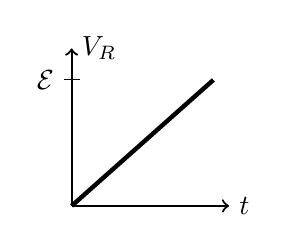
\begin{tikzpicture}
      \draw[thick,->](0,0)--(2,0)node[right]{$t$};
      \draw[thick,->](0,0)--(0,2)node[right]{$V_R$};
      \draw[ultra thick](0,0)--(1.8,1.6);
      \draw(.1,1.6)--(-.1,1.6) node[left]{$\mathcal E$};
    \end{tikzpicture}

    \choice
    \hspace{-.2in}
    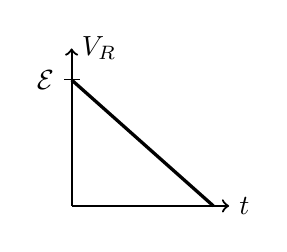
\begin{tikzpicture}
      \draw[thick,->](0,0)--(2,0)node[right]{$t$};
      \draw[thick,->](0,0)--(0,2)node[right]{$V_R$};
      \draw[very thick](0,1.6)--(1.8,0);
      \draw(.1,1.6)--(-.1,1.6) node[left]{$\mathcal E$};
    \end{tikzpicture}

    \choice
    \hspace{-.2in}
    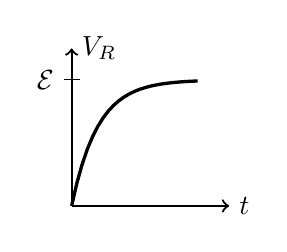
\begin{tikzpicture}
      \draw[thick,->](0,0)--(2,0)node[right]{$t$};
      \draw[thick,->](0,0)--(0,2)node[right]{$V_R$};
      \draw(.1,1.6)--(-.1,1.6) node[left]{$\mathcal E$};
      \draw[very thick,domain=0:1.6] plot(\x,{1.6*(1-exp(-3*\x))});
    \end{tikzpicture}

    \choice
    \hspace{-.2in}
    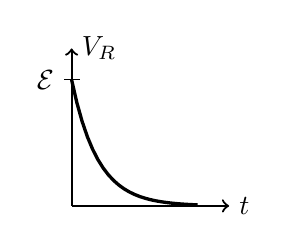
\begin{tikzpicture}
      \draw[thick,->](0,0)--(2,0)node[right]{$t$};
      \draw[thick,->](0,0)--(0,2)node[right]{$V_R$};
      \draw(.1,1.6)--(-.1,1.6) node[left]{$\mathcal E$};
      \draw[very thick,domain=0:1.6] plot(\x,{1.6*exp(-3*\x))});
    \end{tikzpicture}

    \choice
    \hspace{-.2in}
    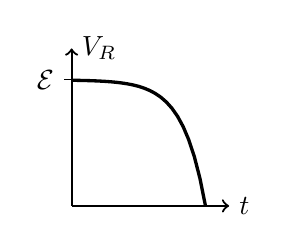
\begin{tikzpicture}
      \draw[thick,->](0,0)--(2,0)node[right]{$t$};
      \draw[thick,->](0,0)--(0,2)node[right]{$V_R$};
      \draw(.1,1.6)--(-.1,1.6) node[left]{$\mathcal E$};
      \draw[very thick,domain=0:1.7] plot(\x,{1.6*(1-exp(3.5*(\x-1.7)))});
    \end{tikzpicture}
  \end{oneparchoices}
  \vspace{.6in}
  
  \uplevel{\rule{\linewidth}{.5pt}}

  \uplevel{
    \textbf{Question \ref{rcirc1}--\ref{rcirc2}}
    \cpic{.35}{r-circuit1}

    \vspace{-.1in}An electric circuit consists of a \SI{12}{\volt} battery, an
    ideal \SI{10}{\ampere} fuse, and three \SI2{\ohm} resistors connected as
    shown above.
    }
  \question What would be the reading on a voltmeter connected across points
  $A$ and $C$?
  \label{rcirc1}
  \begin{choices}
    \choice\SI{12}\volt
    \choice\SI6\volt
    \choice\SI3\volt
    \choice\SI2\volt
    \choice\SI0\volt, since the fuse would break the circuit
  \end{choices}

  \question What would be the reading on an ammeter inserted at point $B$?
  \label{rcirc2}
  \begin{choices}
    \choice\SI9\ampere
    \choice\SI6\ampere
    \choice\SI3\ampere
    \choice\SI2\ampere
    \choice\SI0\ampere, since the fuse would break the circuit
  \end{choices}
  
%  \question A fixed voltage is applied across the length of a tungsten wire. An
%  increase in the power dissipated by the wire would result if which of the
%  following could be increased?
%  \begin{choices}
%    \choice The resistivity of the tungsten
%    \choice The cross-sectional area of the wire
%    \choice The length of the wire
%    \choice The temperature of the wire
%    \choice The temperature of the wire’s surroundings
%  \end{choices}

  \uplevel{
    \rule{\linewidth}{.5pt}
    \cpic{.24}{3-bulbs}
  }

  \question The three light bulbs in the circuit below are identical, and the
  battery has zero internal resistance. When switch $S$ is closed to cause
  bulb 1 to light, which of the other two bulbs increase(s) in brightness?

  \begin{minipage}{.3\linewidth}
    \pic{.75}{3-bulbs}
  \end{minipage}
  \begin{minipage}{.64\linewidth}
    \begin{choices}
      \choice Neither bulb
      \choice Bulb 2 only
      \choice Bulb 3 only
      \choice Both bulbs
      \choice It cannot be determined without knowing the emf of the battery.
    \end{choices}
  \end{minipage}
  
  \uplevel{ \rule{\linewidth}{.5pt}}
    
  \question A length of wire of resistance $R$ is connected across a battery
  with zero internal resistance. The wire is then cut in half and the two
  halves are connected in parallel. When the combination is reconnected across
  the battery, what happens to the resultant power dissipated and the current
  drawn from the battery?

  \begin{tabular}{cll}
    & \underline{Power} & \underline{Current}\\
    (A) & No change  & No change \\
    (B) & Doubles    & Doubles   \\
    (C) & Quadruples & Doubles   \\
    (D) & Doubles    & Quadruples\\
    (E) & Quadruples & Quadruples
  \end{tabular}
  
  \uplevel{\rule{\linewidth}{.5pt}}
  
  \question In the circuit shown below, the \SI{10}{\micro\farad} capacitor is
  initially uncharged. After the switch $S$ has been closed for a long time,
  how much energy is stored in the capacitor?

  \begin{minipage}{.4\linewidth}
    \begin{tikzpicture}[scale=1.3]
      \draw[very thick](1.2,0) to[short,*-] (0,0)
      to[battery1,l=\SI{10}\volt] (0,2) to[R,l=\SI5\ohm] (3,2)
      to [C,l=\SI{10}{\micro\farad}] (3,0) to[short,-*](1.8,0);
      \draw[very thick,rotate around={30:(1.2,0)}](1.2,0)--(1.8,0)
        node[above]{$S$};
    \end{tikzpicture}
  \end{minipage}
  \begin{minipage}{.54\linewidth}
    \begin{choices}
      \choice\SI0{\micro\joule}
      \choice\SI{100}{\micro\joule}
      \choice\SI{250}{\micro\joule}
      \choice\SI{500}{\micro\joule}
      \choice\SI{1000}{\micro\joule}
    \end{choices}
  \end{minipage}
  \newpage
  
  \question An electron $e^-$ moving in the plane of the page is injected into a
  uniform magnetic field $\vec B$ that is perpendicular to the page, as shown
  below. Upon entering the field, the electron takes a path that is

  \vspace{.1in}
  \begin{minipage}{.4\linewidth}
    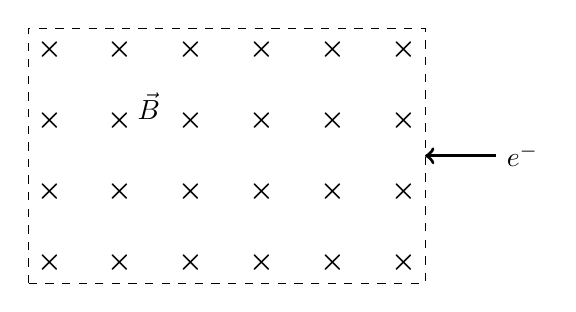
\begin{tikzpicture}[scale=.9]
      \foreach \x in {0,...,5}{
        \foreach \y in {0,...,3} \node at (\x,\y){$\bm\times$};
      }
      \draw[dashed](-.3,-.3) rectangle(5.3,3.3);
      \node at (1.4,2.2){$\vec B$};
      \draw[very thick,<-](5.3,1.5)--(6.3,1.5)node[right]{$e^-$};
    \end{tikzpicture}
  \end{minipage}
  \begin{minipage}{.55\linewidth}
    \begin{choices}
      \choice straight through the field
      \choice clockwise, circular, and in the plane of the page
      \choice counterclockwise, circular, and in the plane of the page
      \choice circular and curved out of the page
      \choice circular and curved into the page
    \end{choices}
  \end{minipage}
  \vspace{.6in}
  
  \uplevel{
    \centering
    \rule{\linewidth}{.5pt}

    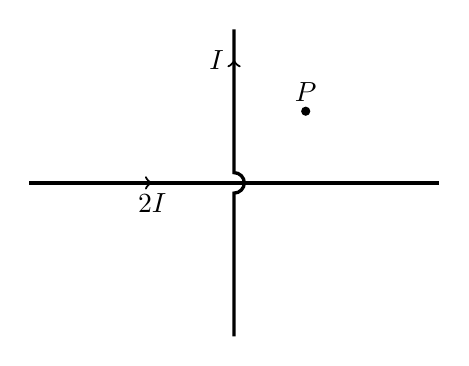
\begin{tikzpicture}[scale=1.3]
      \draw[very thick](0,-1.5)--(0,-.1) arc(-90:90:.1)--(0,1.5);
      \draw[very thick](-2,0)--(2,0);
      \fill(.7,.7) circle(.045) node[above]{$P$};
      \draw[thick,->](-1.2,0)--(-.8,0) node[below]{$2I$};
      \draw[thick,->](0,.8)--(0,1.2) node[left]{$I$};
    \end{tikzpicture}
  }
  \question In the figure above, two long, straight, insulated wires at right
  angles in the plane of the page carry currents of $I$ and $2I$, as shown.
  What is the direction of the magnetic field at point $P$, which is
  equidistant from the wires and coplanar with them?
  \begin{choices}
    \choice Into the page
    \choice Out of the page
    \choice {\huge$\searrow$}
    \choice {\huge$\nwarrow$}
    \choice {\huge$\nearrow$}
  \end{choices}
  
  \uplevel{
    \rule{\linewidth}{.5pt}
    \textbf{Questions \ref{contour1}--\ref{contour2}}
    \cpic{.37}{contours}
    A fixed charge distribution produces the equipotential lines shown in the
    figure above.
  }
  \question Which of the following expressions best represents the magnitude of
  the electric field at point $P$?
  \label{contour1}
  \begin{choices}
    \choice $\dfrac{\SI{10}{\volt}}{\SI{.14}{\metre}}$
    \choice $\dfrac{\SI{10}{\volt}}{\SI{.04}{\metre}}$
    \choice $\dfrac{\SI{25}{\volt}}{\SI{.14}{\metre}}$
    \choice $\dfrac{\SI{25}{\volt}}{\SI{.04}{\metre}}$
    \choice $\dfrac{\SI{40}{\volt}}{\SI{.25}{\metre}}$
  \end{choices}

  \question The direction of the electric field at point $P$ is most nearly
  \label{contour2}
  \begin{choices}
    \choice toward the left
    \choice toward the right
    \choice toward the bottom of the page
    \choice toward the top of the page
    \choice perpendicular to the plane of the page
  \end{choices}

  \uplevel{ \rule{\linewidth}{.5pt}}
  
  \question A helium nucleus (charge $+2q$ and mass $4m$) and a lithium nucleus
  (charge $+3q$ and mass $7m$) are accelerated through the same electric
  potential difference, $V_0$. What is the ratio of their resultant
  kinetic energies, $\dfrac{K_\text{Li}}{K_\text{He}}$?
  \begin{choices}
    \choice$\dfrac23$
    \choice$\dfrac67$
    \choice 1
    \choice$\dfrac76$
    \choice$\dfrac32$
  \end{choices}
  \newpage
  
  \question The electric potential in the $xy$-plane in a certain region of
  space is given by $V(x,y)=6x^2y-2y^3$, where $x$ and $y$ are in meters and
  $V$ is in volts. What is the magnitude of the $y$-component of the electric
  field at the point $(-1,2)$?
  \begin{choices}
    \choice\SI{0}{\volt\per\metre}
    \choice\SI{4}{\volt\per\metre}
    \choice\SI{18}{\volt\per\metre}
    \choice\SI{24}{\volt\per\metre}
    \choice\SI{30}{\volt\per\metre}
  \end{choices}

  \uplevel{ \rule{\linewidth}{.5pt}}
  
  \uplevel{
    \centering
    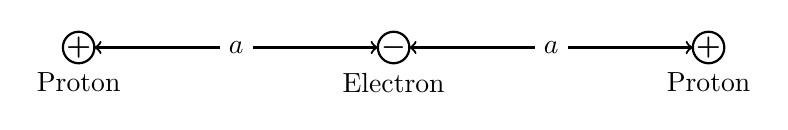
\begin{tikzpicture}
      \draw[thick](-4,0) circle(.2) node{$\bm +$};
      \draw[thick] circle(.2) node{$\bm -$};
      \draw[thick]( 4,0) circle(.2) node{$\bm +$};
      \draw[thick,<->](-3.8,0)--(-.2,0) node[midway,fill=white]{$a$};
      \draw[thick,<->]( 3.8,0)--( .2,0) node[midway,fill=white]{$a$};
      \node[below] at (-4,-.2){Proton};
      \node[below] at ( 0,-.2){Electron};
      \node[below] at ( 4,-.2){Proton};
    \end{tikzpicture}
  }

  \question Two protons and an electron are assembled along a line, as shown
  below. The distance between the electron and each proton is $a$. What is the
  work done by an external force in assembling this configuration of charges?
  \begin{choices}
    \choice $-2\dfrac{ke^2}a$
    \choice $-\dfrac32\dfrac{ke^2}a$
    \choice $\dfrac12\dfrac{ke^2}a$
    \choice $\dfrac32\dfrac{ke^2}a$
    \choice $3\dfrac{ke^2}a$
  \end{choices}

  \uplevel{
    \rule{\linewidth}{.5pt}
    \textbf{Questions \ref{rain1}--\ref{rain2}}

    A cloud contains spherical drops of water of radius $R$ and charge $Q$.
    Assume the drops are far apart.
  }

  \question The electric field $E_0$ and potential $V_0$ at the surface of each
  drop is given by which of the following?
  \label{rain1}
  
  \begin{tabular}{ccc}
    & $E_0$ & $V_0$ \\ \hline
    (A) & 0 & 0 \\
    (B) & $\dfrac{kQ}R$ & $\dfrac{kQ}{R^2}$ \\
    (C) & $\dfrac{kQ}{R^2}$ & $\dfrac{kQ}R$ \\
    (D) & 0 & $\dfrac{kQ}R$ \\
    (E) & $\dfrac{kQ}R$ & 0
  \end{tabular}

  \question If two droplets happen to combine into a single larger droplet, the
  new potential $V$ at the surface of the larger droplet is most nearly equal to
  \label{rain2}
  \begin{choices}
    \choice $3V_0$
    \choice $2V_0$
    \choice $\dfrac2{2^{1/3}}V_0$
    \choice $2^{1/3}V_0$
    \choice $V_0$
  \end{choices}
  
%  \question A point charge $-Q$ is located at the origin, while a second point
%  charge $+2Q$ is located at $x=d$ on the $x$-axis, as shown above. A point on
%  the $x$-axis where the net electric field is zero is located in which of the
%  following regions?
%
%  \vspace{.1in}
%  \begin{minipage}{.3\linewidth}
%    \begin{tikzpicture}
%      \draw[very thick,->](-1,0)--(3,0) node[right]{$x$};
%      \draw(0,.1)--(0,-.1) node[below]{0};
%      \draw(1,.1)--(1,-.1) node[below]{$\dfrac{d}2$};
%      \draw(2,.1)--(2,-.1) node[below]{$d$};
%      \fill circle(.05) node[above]{$-Q$};
%      \fill(2,0) circle(.05) node[above]{$+2Q$};
%    \end{tikzpicture}
%  \end{minipage}
%  \begin{minipage}{.4\textwidth}
%    \begin{choices}
%      \choice $-\infty<x<0$
%      \choice $0<x<\dfrac{d}2$
%      \choice $\dfrac{d}2<x<d$
%      \choice $d<x<\infty$
%      \choice No region on the $x$-axis
%    \end{choices}
%  \end{minipage}
%  
  \uplevel{ \rule{\linewidth}{.5pt}}
  
  \question An inductor of inductance $L$ is connected in series with a
  resistor of resistance $R$, a battery of emf $\mathcal E$, and a switch, as
  shown above. When the switch is closed, the current $I$ in the circuit
  increases with time, approaching the value $I_\text{max}$. What is
  $I_\text{max}$?
  
  \begin{minipage}{.4\textwidth}
    \begin{tikzpicture}[scale=1.2]
      \draw[thick](2.3,2) to[short,*-](4,2) to[R,l=$R$](4,0) to[L,l=$L$](0,0)
      to[battery1,l=$\mathcal E$] (0,2) to[short,-*](1.7,2)--(2.3,2.2);
    \end{tikzpicture}
  \end{minipage}
  \begin{minipage}{.4\linewidth}
    \begin{choices}
      \choice $R/L\mathcal E$
      \choice $RL/\mathcal E$
      \choice $\mathcal E/RL$
      \choice $\mathcal E/R$
      \choice $L\mathcal E$
    \end{choices}
  \end{minipage}
  
  
  \uplevel{
    \rule{\linewidth}{.5pt}
    \textbf{Questions \ref{emf1}--\ref{emf2}}
    
    An emf of \SI{20}{\volt} is induced around a metal ring by increasing a
    uniform magnetic field at a constant rate from zero to a final magnitude
    of \SI{1.0e-2}{\tesla} throughout the region enclosed by the ring. The field
    direction is perpendicular to the plane of the ring.
  }
  
  \question If the area enclosed by the ring is \SI{4.0e-3}{\metre\squared},
  what is the time interval during which the field is increased?
  \label{emf1}
  \begin{choices}
    \choice \SI{2.}{\micro\second}
    \choice \SI{5.}{\micro\second}
    \choice \SI{10}{\micro\second}
    \choice \SI{20}{\micro\second}
    \choice \SI{50}{\micro\second}
  \end{choices}

  \question If the electrical resistance of the ring is \SI{500}\ohm, what is
  the rate at which energy is dissipated in the ring as the field is increased?
  \label{emf2}
  \begin{choices}
    \choice\SI{.040}\watt
    \choice\SI{.80}\watt
    \choice\SI{1.25}\watt
    \choice\SI{25}\watt
    \choice\SI{1.e4}\watt
  \end{choices}

  
  \uplevel{
    \centering
    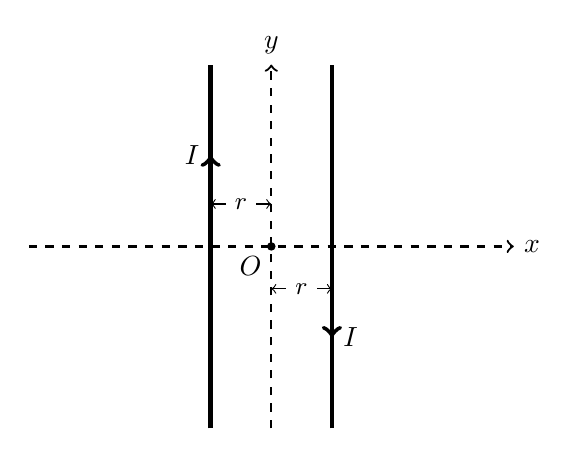
\begin{tikzpicture}[scale=.77]
      \draw[dashed,thick,->](-4,0)--(4,0)node[right]{$x$};
      \draw[dashed,thick,->](0,-3)--(0,3)node[above]{$y$};
      \draw[ultra thick](-1,-3)--(-1,3);
      \draw[ultra thick]( 1,-3)--( 1,3);
      \draw[<->](-1,.7)--(0,.7)  node[midway,fill=white]{\small$r$};
      \draw[<->](1,-.7)--(0,-.7) node[midway,fill=white]{\small$r$};
      \draw[ultra thick,->](-1,0)--(-1,1.5) node[left]{$I$};
      \draw[ultra thick,->](1,0)--(1,-1.5) node[right]{$I$};
      \fill circle(.07) node[below left]{$O$};
    \end{tikzpicture}
    \hspace{.3in}
    \begin{tikzpicture}[scale=.77]
      \draw[dashed,thick,->](-4,0)--(4,0)node[right]{$x$};
      \draw[dashed,thick,->](0,-3)--(0,3)node[above]{$y$};
      \draw[ultra thick](-4,0)--(-1,0)--(-1,3);
      \draw[ultra thick](3.8,0)--(1,0)--(1,-3);
      \draw[<->](-1,.7)--(0,.7)  node[midway,fill=white]{\small$r$};
      \draw[<->](1,-.7)--(0,-.7) node[midway,fill=white]{\small$r$};
      \draw[ultra thick,->](-1,0)--(-1,1.5) node[left]{$I$};
      \draw[ultra thick,->](-3,0)--(-2.3,0);
      \draw[ultra thick,->](1,0)--(1,-1.5) node[right]{$I$};
      \draw[ultra thick,->](3,0)--(2.3,0);
      \fill circle(.07) node[below left]{$O$};
    \end{tikzpicture}
  }

  \question Two long, straight wires are parallel to and equidistant from the
  $y$-axis, as shown above left. Each carries current $I$ in opposite
  directions, resulting in a magnetic field of magnitude $B_0$ at the origin.
  If the wires are each bent into right angles and placed as shown above right,
  what is the magnitude of the magnetic field $B$ at the origin?
  \begin{choices}
    \choice Zero
    \choice Between zero and $B_0/2$
    \choice $B_0/2$
    \choice Between $B_0/2$ and $B_0$
    \choice $B_0$
    \end{choices}

  \uplevel{
    \centering
    \rule{\linewidth}{.5pt}

    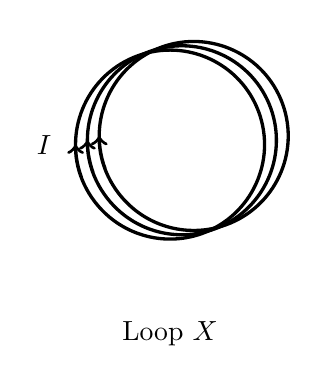
\begin{tikzpicture}[scale=.8]
      \begin{scope}[rotate=20,very thick,->]
        \draw(-1.5,0) arc(180:-200:1.5);
        \draw(-1.3,0) arc(180:-200:1.5);
        \draw(-1.1,0) arc(180:-200:1.5);
      \end{scope}
      \node at (-2,0) {$I$};
      \node at (0,-3) {Loop $X$};
    \end{tikzpicture}
    \hspace{.3in}
    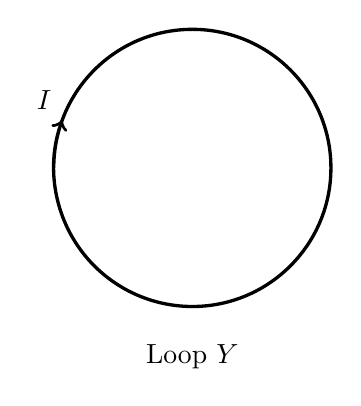
\begin{tikzpicture}[scale=.8]
      \draw[very thick,->](-2.2,0) arc(180:-200:2.2) node[above left]{$I$};
      \node at (0,-3) {Loop $Y$};
    \end{tikzpicture}
  }

  \question A length of wire carrying a steady clockwise current $I$ is bent
  to form the triple circular loop $X$ above. An identical length of the same
  wire is bent less tightly to form the single loop $Y$ of larger radius, which
  carries the same current $I$. The ratio of the magnetic field strength at the
  center of loop $Y$ to the magnetic field strength at the center of loop $X$ is
  \begin{choices}
    \choice $1/9$
    \choice $1/3$
    \choice 1
    \choice 3
    \choice 9
  \end{choices}
  
  \uplevel{
    \rule{\linewidth}{.5pt}
    \cpic{.26}{cable-xsection}
  }
  \question The diagram above shows the cross section of a long cable that has
  an inner wire of radius $R$ surrounded by a conducting sheath of outer radius
  $2R$. The wire and the sheath carry currents in opposite directions but with
  the same uniform current density $J$. What is the magnitude of the magnetic
  field at the surface of the outer conductor?
  \begin{choices}
    \choice Zero
    \choice $\dfrac14\mu_0RJ$
    \choice $\dfrac12\mu_0RJ$
    \choice $\dfrac34\mu_0RJ$
    \choice $\mu_0RJ$
  \end{choices}

  \uplevel{
    \uplevel{\rule{\linewidth}{.5pt}}
    \cpic{.2}{long-wire1}
  }
  \question A long wire of radius $R$ carries a current $I$, as
  shown above, with a current density $J=ar$ that increases linearly with the
  distance $r$ from the center of the wire. Which of the following graphs best
  represents the magnitude of the magnetic field $B$ as a function $r$?

  \begin{oneparchoices}
    \choice
    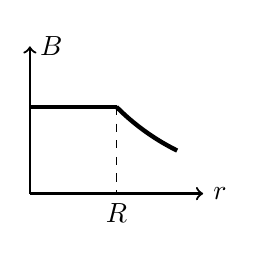
\begin{tikzpicture}[scale=1.1]
      \draw[thick,->](0,0)--(2,0)  node[right]{$r$};
      \draw[thick,->](0,0)--(0,1.7)node[right]{$B$};
      \draw[dashed](1,1)--(1,0) node[below]{$R$};
      \draw[ultra thick](0,1)--(1,1);
      \draw[ultra thick,domain=1:1.7] plot(\x,{2.72*exp(-\x)});
    \end{tikzpicture}

    \choice
    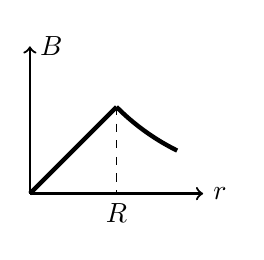
\begin{tikzpicture}[scale=1.1]
      \draw[thick,->](0,0)--(2,0)  node[right]{$r$};
      \draw[thick,->](0,0)--(0,1.7)node[right]{$B$};
      \draw[dashed](1,1)--(1,0) node[below]{$R$};
      \draw[ultra thick](0,0)--(1,1);
      \draw[ultra thick,domain=1:1.7] plot(\x,{2.72*exp(-\x)});
    \end{tikzpicture}

    \choice
    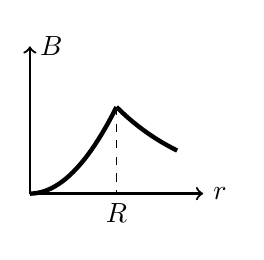
\begin{tikzpicture}[scale=1.1]
      \draw[thick,->](0,0)--(2,0)  node[right]{$r$};
      \draw[thick,->](0,0)--(0,1.7)node[right]{$B$};
      \draw[dashed](1,1)--(1,0) node[below]{$R$};
      \draw[ultra thick,domain=0:1]   plot(\x,{\x*\x)});
      \draw[ultra thick,domain=1:1.7] plot(\x,{2.72*exp(-\x)});
    \end{tikzpicture}

    \choice
    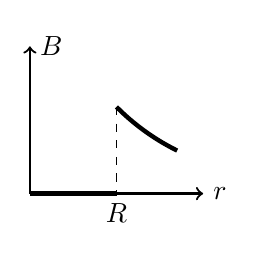
\begin{tikzpicture}[scale=1.1]
      \draw[thick,->](0,0)--(2,0)  node[right]{$r$};
      \draw[thick,->](0,0)--(0,1.7)node[right]{$B$};
      \draw[dashed](1,1)--(1,0) node[below]{$R$};
      \draw[ultra thick](0,0)--(1,0);
      \draw[ultra thick,domain=1:1.7] plot(\x,{2.72*exp(-\x)});
    \end{tikzpicture}

    \choice
    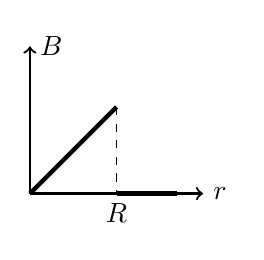
\begin{tikzpicture}[scale=1.1]
      \draw[thick,->](0,0)--(2,0)  node[right]{$r$};
      \draw[thick,->](0,0)--(0,1.7)node[right]{$B$};
      \draw[dashed](1,1)--(1,0) node[below]{$R$};
      \draw[ultra thick] (0,0)--(1,1);
      \draw[ultra thick] (1,0)--(1.7,0);
    \end{tikzpicture}    
  \end{oneparchoices}
  \vspace{.3in}
  \newpage
  
  \question In the circuit drawn above, the switch $S$ is initially open, and
  the capacitor $C$ is charged with the polarity indicated. The switch is then
  closed, and the capacitor begins discharging through the resistor. Which of
  the following is true of the current that is subsequently induced in the
  circular wire loop near the long, straight wire $AB$?

  \begin{minipage}{.3\linewidth}
    \pic{.8}{rc-loop}
  \end{minipage}
  \begin{minipage}{.59\linewidth}
    \begin{choices}
      \choice It is counterclockwise and constant.
      \choice It is counterclockwise and increases with time.
      \choice It is counterclockwise and decreases with time.
      \choice It is clockwise and increases with time.
      \choice It is clockwise and decreases with time
    \end{choices}
  \end{minipage}
  \vspace{.3in}
  
  \uplevel{\rule{\linewidth}{.5pt}}
  
  \question Which of the following statements contradicts one of Maxwell's
  equations?
  \begin{choices}
    \choice A changing magnetic field produces an electric field.
    \choice A changing electric field produces a magnetic field.
    \choice The net magnetic flux through a closed surface depends on the
    current inside.
    \choice The net electric flux through a closed surface depends on the
    charge inside.
    \choice The electric field due to an isolated stationary point charge is
    inversely proportional to the square of the distance from the charge.
  \end{choices}
  \vspace{.7in}

  \uplevel{\rule{\linewidth}{.5pt}}
  
  \question A student building a circuit wishes to increase the frequency of an
  oscillator consisting of a capacitor of capacitance $C$ and an inductor of
  inductance $L$. Which of the following would accomplish this objective?
  \begin{enumerate}[nosep,label={\Roman*.}]
  \item Increase $L$
  \item Increase $C$
  \item Decrease $L$
  \item Decrease $C$
  \end{enumerate}
  \vspace{.2in}
  \begin{choices}
    \choice I only
    \choice I or II
    \choice I or IV
    \choice II or III
    \choice III or IV
  \end{choices}
\end{questions}
\end{document}
